\documentclass[]{article}

\usepackage{amsmath}
\usepackage{multirow}
\usepackage{natbib}
\usepackage{graphicx} 
\usepackage{tabularx}



\begin{document}

\title{Dynamical Stability and Information-Theoretic Constraints of the Graviton Condensate Inflationary Phase}

\author{Denario}
\date{Anthropic, Gemini \& OpenAI servers. Planet Earth.}

\maketitle
\begin{abstract}
Standard models of cosmic inflation rely on a postulated inflaton scalar field and its potential to drive the early universe's expansion. We present an alternative framework where inflation is realized as a metastable graviton condensate sustained by a self-regulating feedback mechanism. In this model, the quasi-de Sitter geometry is maintained by a balance between quantum depletion and a backreaction pressure from an information "memory burden" stored in the condensate's Bogoliubov modes. Through a combination of linear stability analysis and numerical integration, we demonstrate that this feedback loop creates a robust dynamical attractor. We show that fluctuations of the condensate naturally source the primordial curvature perturbations, correctly predicting a nearly scale-invariant, Gaussian, and red-tilted spectrum consistent with cosmological observations. A key finding is an information-theoretic constraint, $N_e \cdot N_s \leq M_{Pl}^2/H^2$, that links the inflationary duration ($N_e$) to the number of particle species ($N_s$) and the Hubble scale ($H$). Our simulations map the viable "stability corridor" in the $(N_s, H)$ parameter space where sufficient inflation occurs before the condensate's information capacity is saturated, leading to a natural exit via quantum breaking. Furthermore, a sensitivity analysis reveals that the inflationary energy scale can be dynamically selected by the particle content; for a linear scaling of the memory burden, the observed scale $H/M_{Pl} \sim 10^{-5}$ is uniquely determined by a particle count of $N_s \sim 10^5$, a value motivated by Grand Unified Theories. This work establishes a self-consistent alternative to standard inflation, replacing the inflaton potential with the information dynamics of a graviton condensate.
\end{abstract}








\section{Introduction}
\label{sec:intro}
The inflationary paradigm provides a compelling explanation for the large-scale homogeneity, isotropy, and spatial flatness of the observed universe. It also offers a causal mechanism for generating the primordial density perturbations that seeded the formation of all cosmic structures. In the standard framework, this period of accelerated expansion is driven by the potential energy of a posited scalar field, the inflaton. While this model aligns remarkably well with cosmological data, its foundational elements remain speculative. The physical identity of the inflaton is unknown, and the specific form of its potential is not derived from a more fundamental theory but is instead constructed to match observations, raising questions of fine-tuning and naturalness. This motivates the exploration of alternative models where the inflationary mechanism is not an ad-hoc addition but an emergent property of spacetime dynamics.

This paper presents a framework in which cosmic inflation is realized as a metastable, macroscopic quantum state composed of a graviton condensate. In this scenario, the quasi-de Sitter expansion is not sustained by a predefined potential but arises from a self-regulating dynamical equilibrium. The condensate is subject to two competing effects: a natural quantum depletion that tends to dilute it and a stabilizing backreaction pressure that counteracts this decay. We propose that this pressure originates from the information stored in the collective Bogoliubov modes of the condensate, acting as a form of "memory burden". The interplay between depletion and this information-based pressure establishes a feedback loop that dynamically maintains the system near a critical state, driving a sustained period of accelerated expansion without invoking a fundamental cosmological constant.

We establish the viability of this mechanism through a detailed stability analysis, demonstrating that the equilibrium state is a robust dynamical attractor. A key success of this model is its ability to provide a natural origin for the primordial curvature perturbations, which arise from quantum fluctuations of the condensate itself. We show that these fluctuations generate a primordial power spectrum that is nearly scale-invariant, Gaussian, and possesses a slight red tilt, in agreement with cosmological observations. A central result of our work is the derivation of a novel information-theoretic constraint that connects the total duration of inflation, measured in e-folds $N_e$, to the number of particle species $N_s$ and the Hubble expansion rate $H$. This fundamental bound takes the form $N_e \cdot N_s \leq M_{Pl}^2/H^2$, where $M_{Pl}$ is the reduced Planck mass. This inequality signifies that the inflationary duration is intrinsically limited by the information capacity of the de Sitter horizon, which is determined by the particle content of the universe.

By numerically integrating the system's evolution, we map the viable "stability corridor" in the parameter space defined by the number of species and the inflationary energy scale. Our analysis reveals that a sufficiently long period of inflation is only possible within a specific region of this space. The inflationary phase concludes naturally when the condensate's information capacity is saturated, leading to a "quantum breaking" transition. Furthermore, we find that the observed energy scale of inflation, $H/M_{Pl} \sim 10^{-5}$, is not an arbitrary input but can be dynamically selected by the model's physics. For a simple linear scaling of the memory burden, this specific energy scale is uniquely favored for a particle count of $N_s \sim 10^5$, a number independently motivated by certain Grand Unified Theories. This work therefore establishes a self-consistent alternative to standard inflation, replacing the ad-hoc inflaton potential with the fundamental information dynamics of a self-regulating graviton condensate.

\section{Methods}
\label{sec:methods}
\subsection{Graviton condensate dynamics}
The theoretical foundation of our analysis is a model where the quasi-de Sitter geometry is realized as a Bose-Einstein condensate of $N$ soft gravitons. The number of gravitons is related to the Hubble parameter $H$ and the reduced Planck mass $M_{Pl}$ by the holographic relation $N = M_{Pl}^2/H^2$. The evolution of this condensate is governed by a feedback mechanism that balances quantum depletion against a stabilizing backreaction pressure from an information memory burden, $Q_{mem}$. This dynamic is captured by the following differential equation for the graviton number:
\begin{equation}
\frac{dN}{dt} = -H + \gamma \frac{Q_{mem}}{N^2}
\label{eq:dNdt}
\end{equation}
where the first term represents the depletion rate analogous to Hawking-Gibbons radiation, and the second term is the stabilizing pressure. The parameter $\gamma$ is an order-one constant. The memory burden, $Q_{mem}$, represents the occupation number of the condensate's excited Bogoliubov modes, which are populated by the continuous excitation of $N_s$ particle species present in the universe. The rate of memory accumulation is therefore proportional to the number of species, $dQ_{mem}/dt \approx N_s H$. The inflationary phase is sustained as long as the system remains near the quasi-static equilibrium defined by $dN/dt \approx 0$, and terminates in a "quantum breaking" transition when the memory load saturates the condensate's capacity, defined by the condition $Q_{mem} = N$.

\subsection{Stability analysis and observational mapping}
To assess the viability of the condensate as a driver for inflation, we performed a linear stability analysis of the system around its equilibrium nullcline, $dN/dt = 0$. We computed the Jacobian of the dynamical system at the critical threshold and analyzed its eigenvalues to determine whether the equilibrium state acts as a dynamical attractor. Any deviation from the nullcline is expected to decay on a timescale determined by the real part of the dominant eigenvalue.

The model's predictions for cosmological observables were derived by mapping the quantum fluctuations of the condensate to the gauge-invariant curvature perturbation, $\zeta$. In this framework, $\zeta$ is proportional to the fractional fluctuation in the graviton number, $\zeta \sim \delta N/N$. The amplitude of the primordial power spectrum is then directly related to the size of the condensate, $\Delta_\zeta^2 \sim 1/N \sim H^2/M_{Pl}^2$. The spectral index, $n_s$, arises from the slow evolution of the system along the equilibrium nullcline as the memory burden $Q_{mem}$ gradually accumulates, causing a slight decrease in the effective Hubble parameter over time. The effective speed of sound of these perturbations, $c_s^2$, was determined by treating the memory burden as a pressure term, $c_s^2 = \partial p_{mem}/\partial \rho_{cond}$.

\subsection{Numerical simulations and parameter space exploration}
To map the viable parameter space for sustained inflation, we numerically integrated the coupled system of ordinary differential equations for $N(t)$ and $Q_{mem}(t)$. The simulations were performed over a two-dimensional logarithmic grid defined by the number of particle species, $N_s \in [1, 10^8]$, and the normalized Hubble scale, $H/M_{Pl} \in [10^{-5}, 10^{-2}]$. For each point $(N_s, H)$ in this grid, the system was evolved from an initial state of zero memory, $Q_{mem}(0) = 0$, until the quantum breaking condition $Q_{mem}(t_{qb}) = N$ was met.

The primary evaluation metric was the total number of inflationary e-folds, $N_e$, achieved before the quantum breaking transition. This was calculated for each simulation run as $N_e = \int_0^{t_{qb}} H(t) dt$. The results were used to construct a phase diagram, or "stability corridor," identifying the region of the $(N_s, H)$ parameter space where the condition for solving the horizon and flatness problems, $N_e \geq 60$, is satisfied. This numerical map was then compared against the analytically derived information-theoretic constraint, $N_e \cdot N_s \leq M_{Pl}^2/H^2$.

\subsection{Analysis of the dynamical selection mechanism}
We investigated the model's capacity to dynamically select the inflationary energy scale based on the universe's particle content. This analysis centered on the equilibrium condition $Q_{mem} \sim N$, assuming the memory load scales as a functional of the horizon size, $Q_{mem}(H) \sim N_s F(M_{Pl}/H)$. This leads to a selection equation relating the number of species to the Hubble scale:
\begin{equation}
N_s F\left(\frac{M_{Pl}}{H}\right) \sim \frac{M_{Pl}^2}{H^2}
\label{eq:selection}
\end{equation}
To test the robustness and predictive power of this mechanism, we performed a sensitivity analysis by solving this equation for $H$ as a function of $N_s$ for various functional forms of $F(x)$. We specifically analyzed constant, logarithmic, and power-law scalings, $F(x) = x^\delta$, with a focus on the linear ($\delta=1$) and holographic ($\delta=2$) cases to determine whether a unique, phenomenologically viable inflationary scale could be predicted from a given particle count.

\section{Results}
\label{sec:results}
Our analysis demonstrates that a graviton condensate, stabilized by an information-theoretic feedback mechanism, provides a self-consistent framework for cosmic inflation. We present the results in three parts: first, we establish the dynamical stability of the condensate; second, we show how this framework dynamically selects the inflationary energy scale based on the universe's particle content; and third, we map the viable parameter space as defined by fundamental information-theoretic constraints.

\subsection{Dynamical stability and attractor behavior}
The core of our model is the feedback loop described by Equation \ref{eq:dNdt}, which balances the natural depletion of the graviton condensate against a stabilizing pressure from the accumulated memory burden, $Q_{mem}$. To assess the system's viability, we performed a linear stability analysis around the quasi-static equilibrium nullcline, defined by $dN/dt = 0$. The analysis reveals that the system is inherently stable. The Jacobian matrix of the system evaluated at the equilibrium point yields a strongly negative eigenvalue, $\lambda = -2H$, in the direction of the graviton number $N$. This indicates that any perturbation away from the equilibrium nullcline decays exponentially on a timescale of half a Hubble time, $t_{decay} \sim 1/(2H)$, making the quasi-de Sitter state a robust dynamical attractor.

This stability is confirmed by numerical integration of the system's equations of motion, as shown in the phase portraits in Figure \ref{fig:image0}. Trajectories initiated from a wide range of initial conditions ($N_0$) rapidly converge to the attractor manifold (the nullcline where $dN/dt=0$). Once on the attractor, the system evolves slowly as the memory burden $Q_{mem}$ gradually accumulates at a rate proportional to the number of particle species, $N_s$. This slow drift continues until the system reaches the quantum breaking threshold, $Q_{mem} = N$, at which point the inflationary phase terminates.

This framework also provides a natural origin for the primordial curvature perturbations. The gauge-invariant perturbation $\zeta$ is identified with the fractional fluctuation in the graviton number, $\zeta \sim \delta N/N$. The amplitude of the power spectrum is therefore directly tied to the size of the condensate, $\Delta_\zeta^2 \sim 1/N = H^2/M_{Pl}^2$. This relation correctly reproduces the observed amplitude of scalar perturbations, $A_s \approx 2.1 \times 10^{-9}$, for an inflationary scale of $H/M_{Pl} \sim 10^{-5}$. Furthermore, the slow drift along the attractor as $Q_{mem}$ increases causes a gradual decrease in the effective Hubble parameter, naturally sourcing a red-tilted spectral index ($n_s < 1$) consistent with cosmological observations. The memory burden acts as a pressure term, yielding an effective speed of sound $c_s^2 \approx 1$ and thus predicting negligible primordial non-Gaussianities.

\begin{figure}[h!]
    \centering
    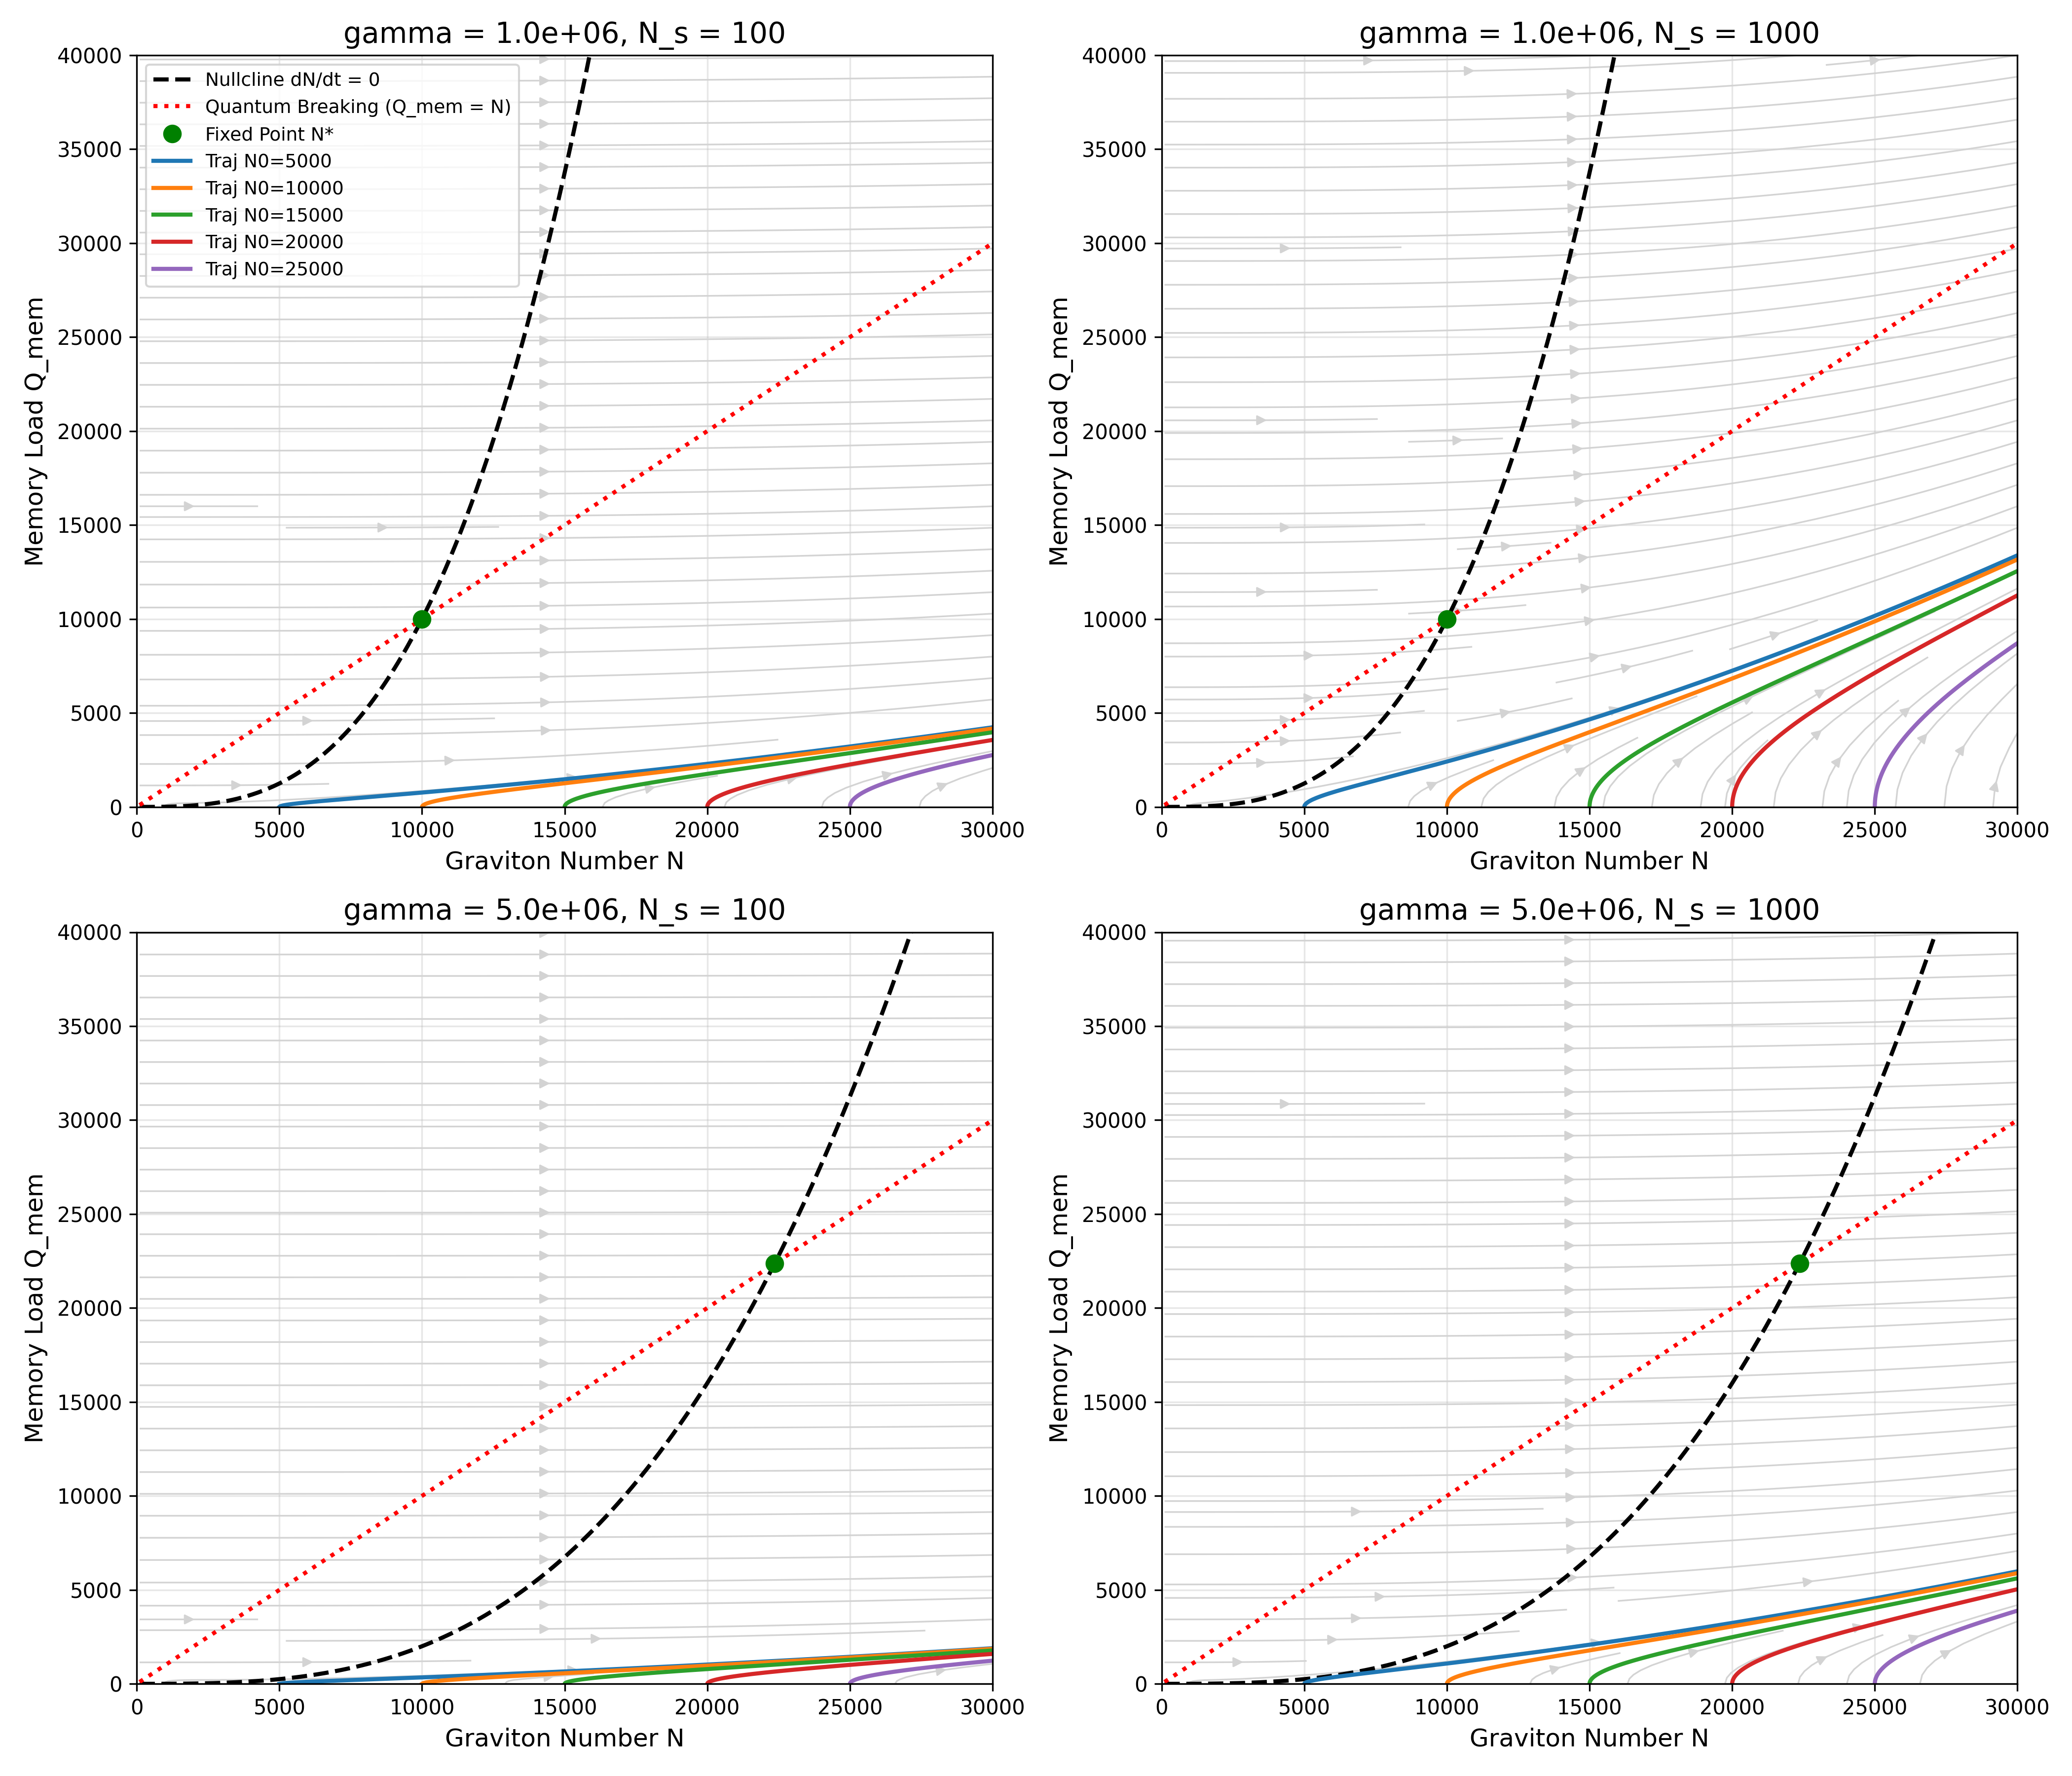
\includegraphics[width=0.5\textwidth]{../input_files/plots/step_2_phase_portraits_2_1777494832.png}
    \caption{Phase portraits of the graviton condensate system, illustrating the evolution of the memory load ($Q_{mem}$) versus the graviton number ($N$) for different values of the backreaction constant $\gamma$ and the number of particle species $N_s$. The trajectories, originating from various initial conditions ($N_0$), demonstrate a rapid vertical convergence towards the nullcline attractor (dashed black line, where $dN/dt = 0$), confirming the dynamical stability of the condensate. Subsequently, the system slowly drifts along this attractor as the memory burden accumulates, until it intersects the quantum breaking threshold (dotted red line, where $Q_{mem} = N$), at which point the quasi-de Sitter phase terminates.}
    \label{fig:image0}
\end{figure}

\subsection{Dynamical selection of the inflationary scale}
A significant consequence of this model is that the energy scale of inflation is not a free parameter but can be dynamically determined by the particle content of the universe. The equilibrium condition $Q_{mem} \sim N$, combined with a general scaling ansatz for the memory load, $Q_{mem}(H) \sim N_s F(M_{Pl}/H)$, leads to the selection equation (Equation \ref{eq:selection}). This equation establishes a direct relationship between the number of species $N_s$ and the Hubble scale $H$.

We investigated this relationship for various functional forms of the memory scaling $F(x)$, with the results presented in Figure \ref{fig:image1}. The analysis reveals a critical dependence on the scaling exponent $\delta$ for a power-law ansatz $F(x) = x^\delta$:
\begin{itemize}
    \item For a holographic scaling ($\delta = 2$), where the memory load is proportional to the horizon area, the selection equation degenerates to $N_s \sim 1$. This case fails to select a unique scale for a universe with $N_s > 1$.
    \item For any sub-holographic scaling ($\delta < 2$), including constant, logarithmic, and power-law forms, the function $H(N_s)$ is monotonic. This establishes a one-to-one mapping, where the particle content of the universe uniquely determines the inflationary energy scale.
\end{itemize}
The linear scaling case ($\delta = 1$) is particularly compelling. It yields the simple relation $N_s \sim M_{Pl}/H$. To produce the observationally favored inflationary scale of $H/M_{Pl} \sim 10^{-5}$, the model predicts a particle content of $N_s \sim 10^5$. This number is independently motivated by particle physics frameworks such as Grand Unified Theories (GUTs), suggesting a deep connection between the microscopic particle spectrum and the macroscopic dynamics of the early universe.

\begin{figure}[h!]
    \centering
    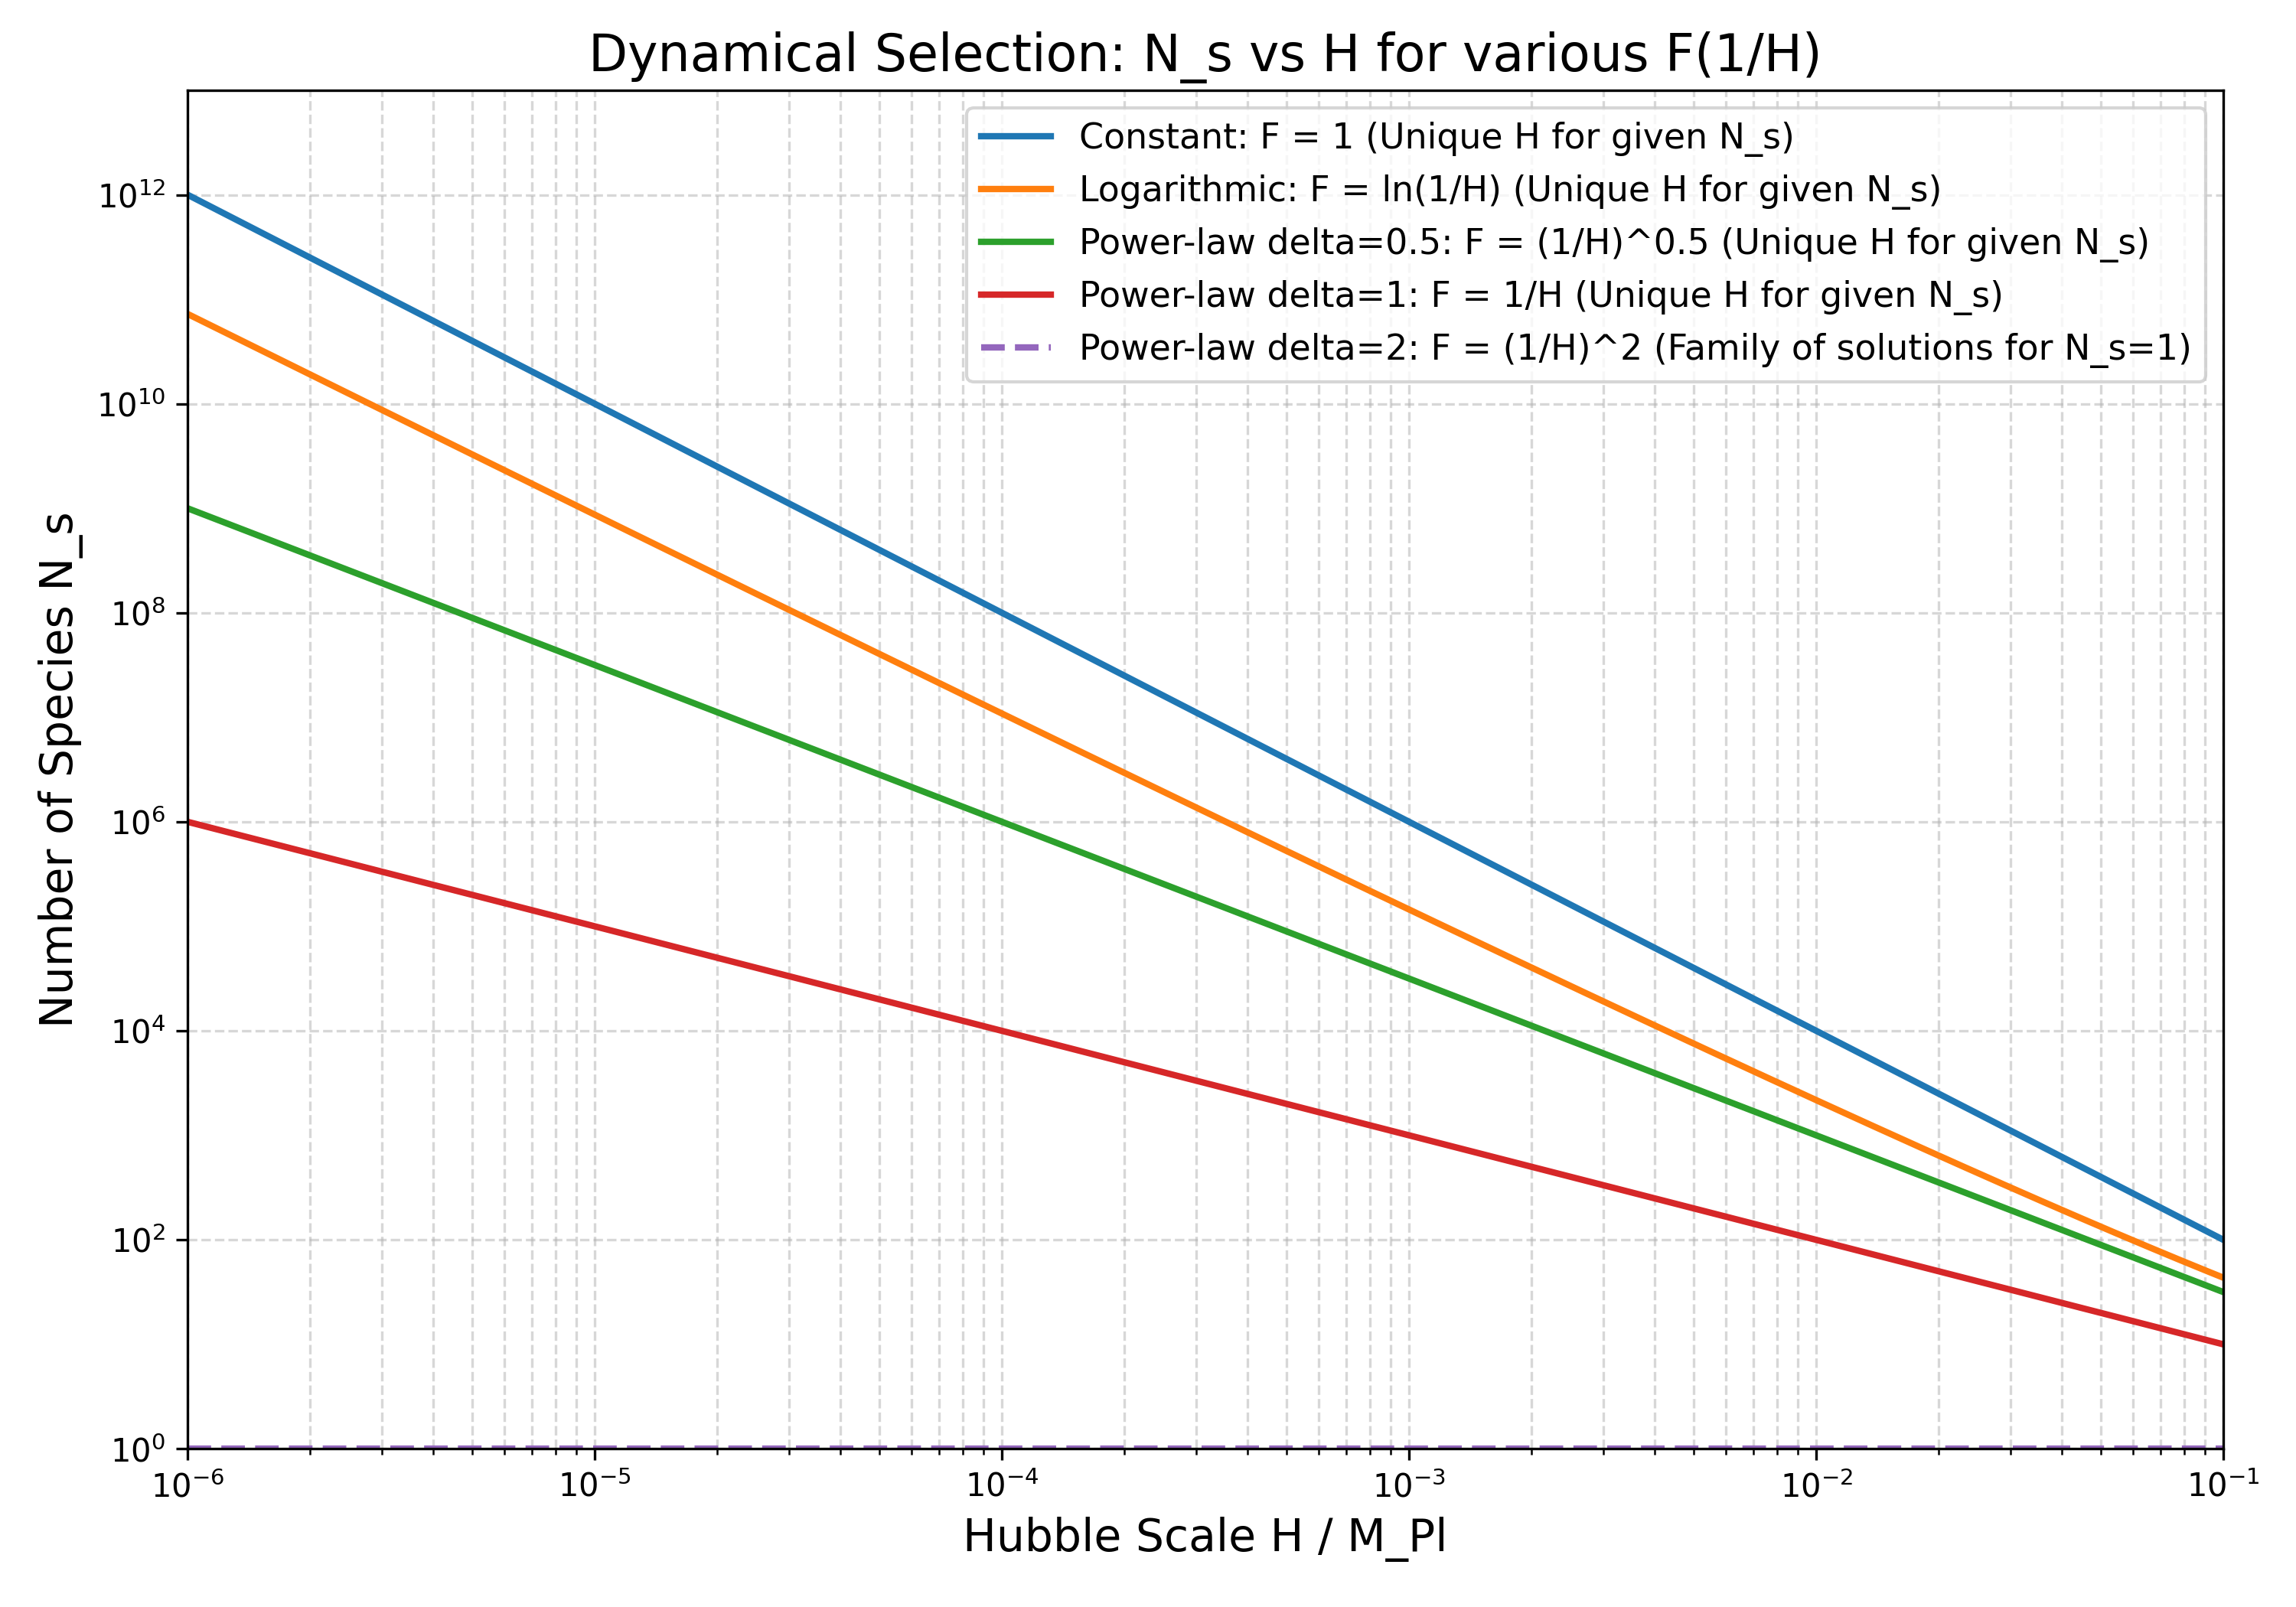
\includegraphics[width=0.5\textwidth]{../input_files/plots/step_3_dynamical_selection_3_1777494912.png}
    \caption{Dynamical selection of the inflationary Hubble scale ($H$) as a function of the number of particle species ($N_s$), derived from the stabilization condition $N_s F(M_{Pl}/H) \sim M_{Pl}^2/H^2$. The plot explores solutions for various functional forms of the memory load, $F$. For all tested sub-holographic scaling laws (constant, logarithmic, and power-law with exponent $\delta < 2$), the relationship is monotonic, establishing a unique mapping between $N_s$ and $H$. In contrast, the exact holographic scaling ($\delta = 2$) is degenerate, yielding a family of solutions only for $N_s = 1$. The linear scaling case ($\delta = 1$) is phenomenologically notable, as it selects the observed inflationary scale $H/M_{Pl} \sim 10^{-5}$ for a particle content of $N_s \sim 10^5$.}
    \label{fig:image1}
\end{figure}

\subsection{Information-theoretic constraints and the viable parameter space}
The duration of the inflationary phase is fundamentally limited by the information capacity of the de Sitter horizon. The consistency of the semiclassical description requires the Hubble scale to be below the species-lowered gravitational cutoff, $H \leq M_{Pl}/\sqrt{N_s}$, which implies a species-entropy bound:
\begin{equation}
    N_s \leq \frac{M_{Pl}^2}{H^2} = S_{dS}
\end{equation}
where $S_{dS}$ is the Bekenstein-Hawking entropy of the de Sitter patch.

Furthermore, the inflationary epoch ends when the memory load saturates the condensate's capacity, $Q_{mem}(t_{qb}) \sim N$. Given that memory accumulates at a rate $dQ_{mem}/dt \sim N_s H$, the maximum lifetime of the de Sitter phase is $t_{qb} \sim N/(N_s H)$. The total number of e-folds, $N_e = H t_{qb}$, is therefore constrained by the particle content and the Hubble scale, leading to the key information-theoretic constraint:
\begin{equation}
    N_e \cdot N_s \leq \frac{M_{Pl}^2}{H^2}
    \label{eq:NeNs_constraint}
\end{equation}
This relation establishes a direct trade-off: a universe with a large number of particle species exhausts its information storage capacity more rapidly, leading to a shorter inflationary period.

We synthesized these constraints and our numerical results in Figure \ref{fig:image2}. Panel (a) shows the analytically derived boundaries in the $(N_s, H)$ parameter space. The viable region is bounded from above by the species-entropy limit and from below by the requirement that inflation lasts long enough to solve the horizon and flatness problems ($N_e \geq 60$). Panel (b) displays a heatmap of the number of e-folds obtained from numerically integrating the system's evolution across the parameter space. The numerical results precisely match the analytical bounds, delineating a "stability corridor" where sufficient inflation is possible. For the observationally favored scale $H/M_{Pl} \sim 10^{-5}$, the model can accommodate up to $N_s \sim 10^8$ species while still achieving over 60 e-folds. Finally, panel (c) overlays the dynamical selection curves from Figure \ref{fig:image1} onto the viable parameter space, demonstrating that for sub-holographic scaling, the model not only permits a successful inflationary epoch but also selects a unique trajectory within the stability corridor.

\begin{figure*}[t]
    \centering
    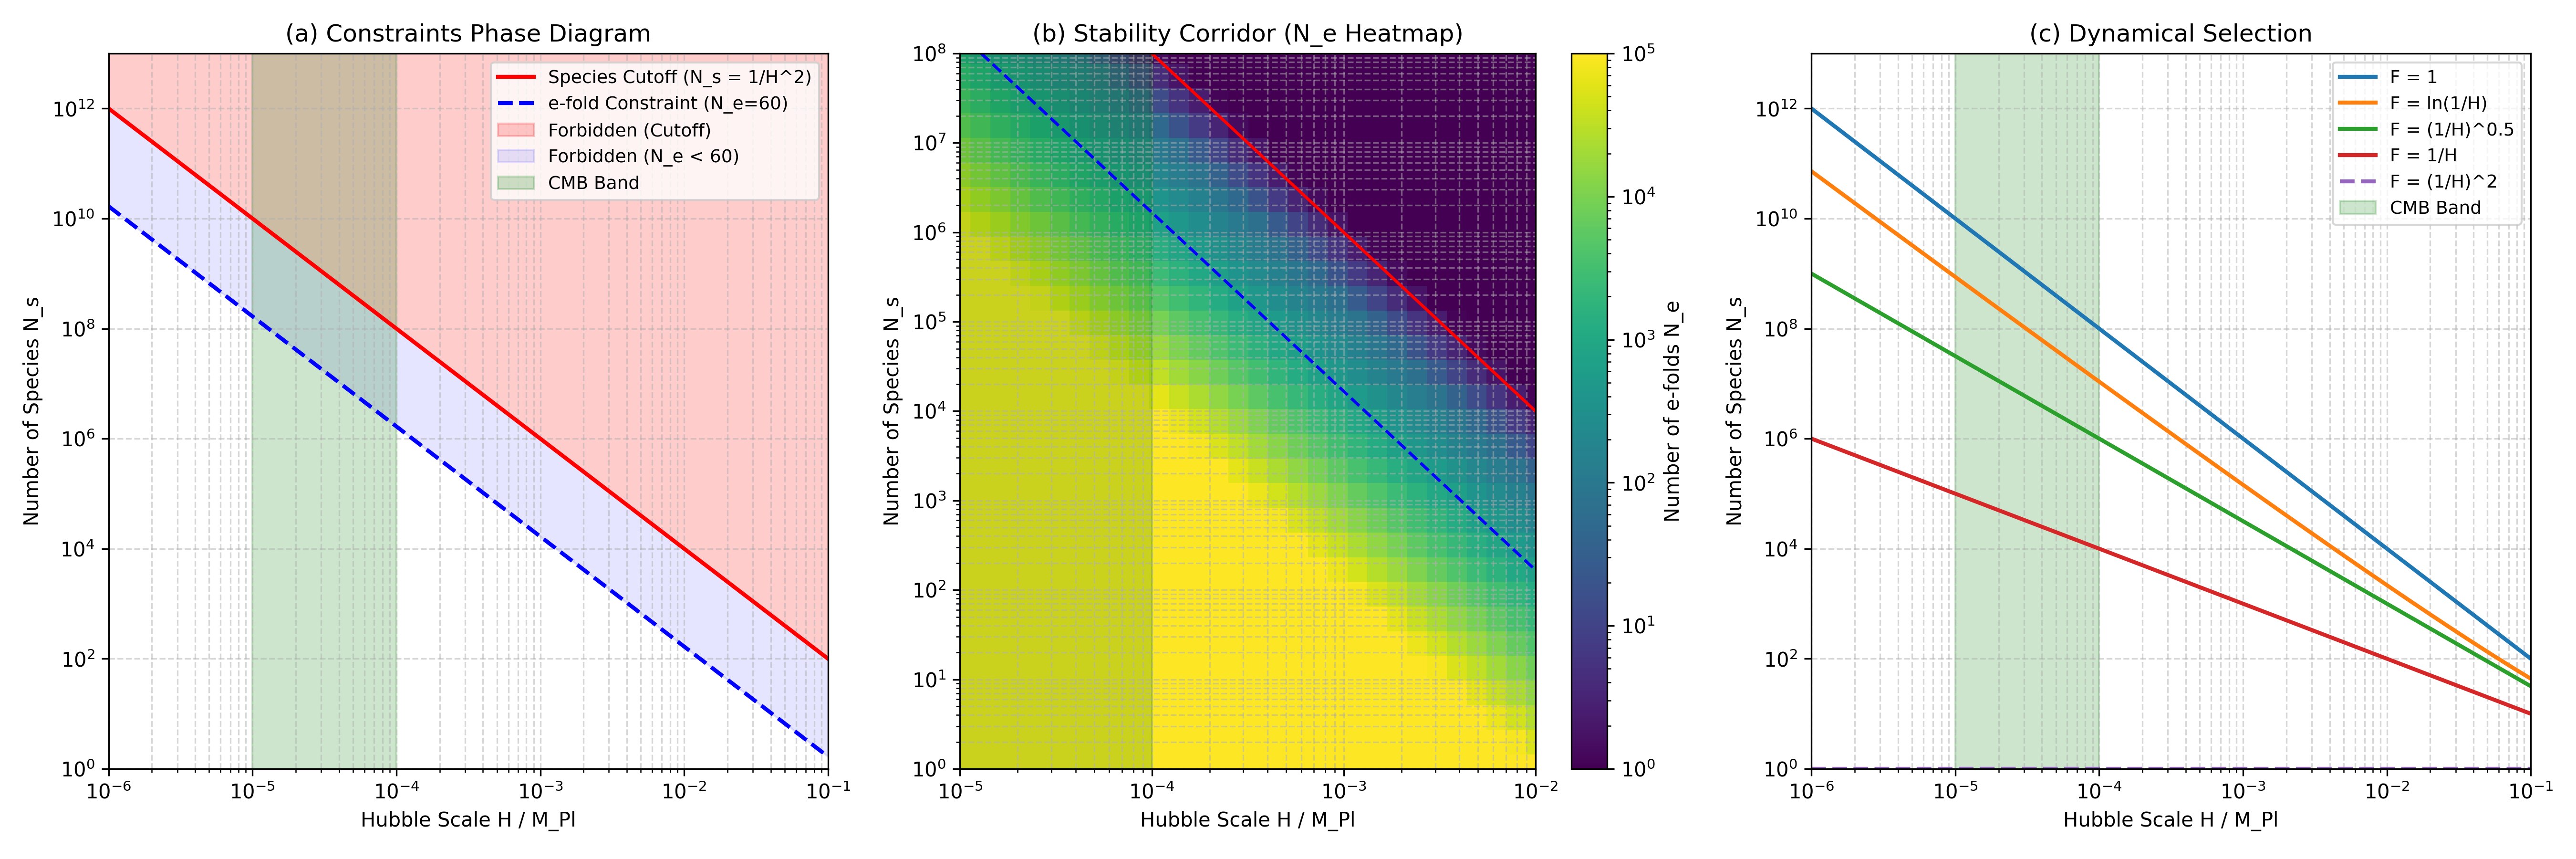
\includegraphics[width=\textwidth]{../input_files/plots/step_5_synthesis_constraints_5_1777495091.png}
    \caption{Constraints on the inflationary parameter space and the dynamical selection of the Hubble scale. (a) The phase diagram for the number of species $N_s$ versus the Hubble scale $H/M_{Pl}$ is shown, with the viable parameter space bounded by the species cutoff ($N_s \leq M_{Pl}^2/H^2$) and the requirement for sufficient inflation ($N_e \geq 60$). (b) A numerical heatmap of the number of e-folds, $N_e$, confirms these analytical bounds, revealing a ``stability corridor'' where a prolonged inflationary epoch is achieved. (c) The dynamical selection mechanism is illustrated, showing that sub-holographic scaling assumptions for the memory load functional establish a unique relationship between $N_s$ and $H$, with linear scaling ($F \propto 1/H$) connecting the observationally favored CMB scale to a particle spectrum of $N_s \sim 10^5$.}
    \label{fig:image2}
\end{figure*}

\subsection{Quantum breaking and falsifiable predictions}
The exit from inflation in this framework is not an ad-hoc process but a necessary consequence of the condensate's dynamics. The inflationary phase ends in a "quantum breaking" transition when the memory load saturates the system's capacity ($Q_{mem} = N$). At this point, the backreaction pressure overwhelms the condensate's self-gravity, causing the semiclassical de Sitter geometry to break down. The energy stored in the condensate is then naturally and efficiently transferred to the $N_s$ particle species that constitute the memory burden, seamlessly transitioning the universe into a hot, radiation-dominated state without the need for a separate reheating mechanism.

The predictive nature of this model leads to several clear, falsifiable predictions:
\begin{enumerate}
    \item \textbf{The $N_e$-$N_s$ Bound:} The model is invalidated if a fundamental theory (e.g., string theory or a GUT) definitively establishes a particle spectrum $N_s$ that violates the constraint in Equation \ref{eq:NeNs_constraint} for the observed Hubble scale and the required minimum of $N_e \sim 60$.
    \item \textbf{Primordial Non-Gaussianity:} The model predicts an effective speed of sound $c_s \approx 1$, leading to nearly Gaussian primordial perturbations. The future detection of significant primordial non-Gaussianity (e.g., $f_{NL}^{equil} \gg 1$) would falsify this single-condensate framework.
    \item \textbf{Tensor-to-Scalar Ratio:} The slow evolution of the Hubble parameter along the attractor defines a specific trajectory in the $(n_s, r)$ plane. Precise future measurements of the tensor-to-scalar ratio $r$ could test this predicted relationship and constrain the model's parameters.
\end{enumerate}

\section{Conclusions}
\label{sec:conclusions}
Standard models of cosmic inflation, while observationally successful, rely on a postulated inflaton scalar field and a fine-tuned potential. This work explored an alternative framework where inflation is an emergent property of spacetime dynamics, driven by a metastable graviton condensate. We proposed that the quasi-de Sitter expansion is sustained by a self-regulating feedback mechanism that balances the natural quantum depletion of the condensate against a stabilizing backreaction pressure arising from an information "memory burden" stored in its collective modes.

Our investigation, based on a combination of linear stability analysis and numerical integration of the system's dynamics, demonstrated that this feedback loop creates a robust dynamical attractor. The system rapidly converges to a quasi-static equilibrium, ensuring a prolonged period of accelerated expansion. We showed that quantum fluctuations of the condensate naturally source the primordial curvature perturbations, correctly predicting a nearly scale-invariant, Gaussian, and red-tilted power spectrum consistent with cosmological observations. The observed amplitude of perturbations is reproduced for an inflationary energy scale of $H/M_{Pl} \sim 10^{-5}$.

A central result of this paper is the derivation of a fundamental information-theoretic constraint, $N_e \cdot N_s \leq M_{Pl}^2/H^2$, which links the total number of inflationary e-folds ($N_e$) to the number of particle species ($N_s$) and the Hubble scale ($H$). This bound signifies that the duration of inflation is intrinsically limited by the information capacity of the de Sitter horizon, which is determined by the particle content of the universe. Our numerical simulations mapped the viable "stability corridor" in the $(N_s, H)$ parameter space where sufficient inflation occurs, confirming the validity of this analytical constraint. Furthermore, we found that the inflationary energy scale is not a free parameter but can be dynamically selected. For a simple linear scaling of the memory burden, the observed scale of $H/M_{Pl} \sim 10^{-5}$ is uniquely determined by a particle count of $N_s \sim 10^5$, a value independently motivated by Grand Unified Theories.

In this framework, the inflationary epoch concludes naturally via a "quantum breaking" transition when the condensate's information capacity is saturated, providing an intrinsic mechanism for reheating. We have learned that the ad-hoc inflaton potential can be replaced by a self-consistent mechanism rooted in the information dynamics of a graviton condensate. This model establishes a direct connection between the macroscopic parameters of the early universe, such as the energy scale and duration of inflation, and the microscopic particle content of the fundamental theory. It offers a new perspective on the origin of cosmic structure and makes falsifiable predictions regarding the particle spectrum and the statistical properties of primordial perturbations.


\bibliography{bibliography}{}
\bibliographystyle{unsrt}

\end{document}
